\chapter{Augmented Reality Tracking Task}
\label{chap:3dtracking}

Portions of this chapter were originally published in the conference proceedings for AIAA Modeling and Simulation Technologies 2019 \citep{karasinski_evaluating_2019}.

\section{Introduction}
\subsection{Overview}
Recent advances in computing hardware have enabled a new generation of mobile augmented reality devices which have the potential to improve human performance and reduce workload in a variety of tasks.
The aim of this study was to investigate the effect of several factors on human performance and workload in a three-axis manual tracking task.
The Microsoft HoloLens is a head-mounted, mobile augmented reality device which provides a stereoscopic 3D view to the user which is not available with traditional 2D displays.
To evaluate whether this new display technology could improve user performance in a tracking task, we designed an experiment that investigated if the depth cueing delivered by stereoscopic display could provide improved performance and decreased workload.
We were also interested to see if a 2D display could gain the benefits of a depth cue by rotating the axis of the task such that the depth cue was more readily available.
Research has also shown that presenting three-dimensional information on a two-dimensional screen is not a simple task, and that the projection of the 3D information onto the 2D screen can cause large changes in the performance of the user~\citep{kim_quantitative_1987}.
In addition to these cues, we also investigated the effects of concurrent bandwidth feedback on task performance and workload as an alternate technique to improving performance.
Concurrent bandwidth feedback alerts the operator when their real-time performance has drifted outside an acceptable, predefined window of performance.
The use of this type of feedback has been shown to improve performance in a wide variety of motor control tasks~\citep{salmoni_knowledge_1984,sigrist_augmented_2013,karasinski_real-time_2017}.

\subsection{Literature Review}
% \subsubsection{Augmented Feedback}
% The concept of feedback was popularized when closed-loop control systems were first developed and has since been defined many times~\citep{Wierner1948}.
% In the context of this work, a convenient definition of feedback comes from Ramaprasad, ``[f]eedback is information about the gap between the actual level and the reference level of a system parameter which is used to alter the gap in some way~\citep{ramaprasad_definition_1983}.''
% The aforementioned ``gap'' is the error and can be conveyed to the operator of a system in a variety of ways.
% Feedback can be broadly classified into two types: intrinsic, feedback which is generated from within the context of the action itself, and extrinsic, feedback which is given from an external source~\citep{laurillard_rethinking_2002}.

% Extrinsic feedback, which is also known as augmented feedback, has been extensively studied in the field motor learning~\citep{sigrist_augmented_2013}.
% In their \citeyear{sigrist_augmented_2013} review, \citeauthor{sigrist_augmented_2013} write ``[i]t is generally accepted that augmented feedback, provided by a human expert or a technical display, effectively enhances motor learning.''
% There are a variety of different forms of augmented feedback, that can be further classified by how, when, and by what form the feedback is provided.
% Concurrent, or real-time, feedback is displayed to the operator while the task is being executed, in contrast to terminal feedback, which is displayed after the task is complete.
% Bandwidth feedback is displayed to the operator when some parameter is inside (on-track feedback) or outside (off-track feedback) of an acceptable, predefined tolerance limit.

% Experimentation with bandwidth feedback traces its origins to \citeauthor{thorndike_law_1927}'s \citeyear{thorndike_law_1927} line-drawing experiment.
% In his experiment, subjects were seated and blindfolded at a table, then asked to draw lines of 3, 4, 5, or 6 inches.
% The experiment was divided into two groups of subjects, one group of subjects received no verbal feedback, while the other group was told ``right'' if they were within an 1/8th of an inch of the desired length for the 3 inch line, or 1/4 of an inch for the other three line lengths, and ``wrong'' if they were outside this bandwidth.
% Subjects that received the verbal bandwidth feedback improved from an initial median ``right'' percentage of 13\% to 54\% after several training sessions.
% The feedback was then removed after these training trials, during which time subjects dropped to a median percentage of 26\%.
% This is consistent with the guidance hypothesis (which was not formalized for another fifty years after this experiment was concluded), which states that consistent feedback during the acquisition phase of learning leads to a dependency on the feedback~\citep{salmoni_knowledge_1984}.
% Subjects became dependent on the verbal feedback (extrinsic feedback) rather than their visual or proprioceptive sense (intrinsic feedback) to such an extent that they could no longer perform with the verbal feedback removed.

% \citeauthor{payne_effect_1955} performed one of the first concurrent bandwidth feedback studies in \citeyear{payne_effect_1955}.
% In their study, subjects completed a multidimensional pursuit test, which required them to scan four simulated aircraft instruments and counter their drift by adjusting simulated aircraft controls.
% Subjects were placed into one of three feedback groups: a control level, where no feedback was provided, a second level, which included a single peripheral visual signal when a deviation in one of the displays occurred, but did not specify which instrument, and a third level, which provided individual indicators for each of the four instruments, and noted the locus of the deviation.
% They found a very significant effect between the different feedback groups, with the control group performing the worst, the second level performing better, and the third level performing better still.
% Subjects completed the test every hour for a four hour period.
% Performance dropped across all three groups as time elapsed and subjects fatigued, but the performance of the subjects in level three was superior at the end of this period compared to the subjects in the control group at the beginning of the experiment.
% They concluded by stating that ``the increment is a positive function of the specificity of the information supplied, it can be ascribed largely to the directive properties of the cues, i.e., the cues impose a more efficient temporal and spatial organization upon [the subject's] scanning behavior~\citep{payne_effect_1955}.''

% \citeauthor{gordon_effect_1967} performed a rotary pursuit study investigating the effects on on-track and off-track concurrent bandwidth feedback in \citeyear{gordon_effect_1967}.
% Subjects in their study were placed into one of three groups: a control, on-track feedback, and off-track feedback.
% The subjects in the bandwidth feedback groups had to track a 0.75 inch by 0.75 inch target with 0.187 inch rigid stylus tip.
% For subjects in the on-track feedback group, a light bulb was illuminated when they were on target, and the light bulb was illuminated for subjects in the off-track group when they were not on the target.
% While both the on-track and off-track groups performed better than the control group, the off-target group performance was slightly superior.
% This finding was consistent with the results \citeauthor{williams_-target_1962} found in a similar task.
% Additionally, subjects in the feedback groups completed several trials at the end of the experiment without feedback and did not experience the loss of performance which is often seen due to the guidance hypothesis.
% This indicates that subjects were able to use the feedback to better learn the task and were not completely dependent on the feedback.
% Subjects used their own intrinsic feedback to learn the task, and were able to take advantage of the concurrent bandwidth feedback to better learn and perform the task without becoming dependent on the external feedback.

% Recent work in the field has taken advantage of modern computing and visualization technology to produce higher fidelity simulations.
% In \citeyear{de_groot_effect_2011}, \citeauthor{de_groot_effect_2011} investigated the effects of concurrent bandwidth feedback on learning a lane-keeping task in a driving simulator.
% Similar to \citeauthor{gordon_effect_1967}, they investigated the effects of on-track and off-track feedback compared to a control group.
% Instead of using a visual indicator, however, de Groot et al. used haptic feedback in the form of a vibrating chair for their feedback groups~\citep{de_groot_effect_2011}.
% They found that on-target and off-target groups had better lane-keeping performance than the control group, and that, similar to \citeauthor{gordon_effect_1967} and \citeauthor{williams_-target_1962}, the off-target group performed best.
% Retention trials, however, showed that a majority of this performance improvement was lost during when the feedback was removed, which was in accordance with the guidance hypothesis.
% The off-target group, though, did still retain some minor performance improvement, which the authors partially attribute to the onset advantage~\citep{fischer_differential_2008}.
% The onset advantage ``suggests that the sudden onset of a stimulus is a more powerful perceptual event than a stimulus offset, facilitating low-level perceptual processing and resulting in faster reaction times~\citep{de_groot_effect_2011}.''
% This effect could explain a repeated finding that off-track feedback is superior to on-track feedback, even if the effect is, in general, small.
% \citeauthor{de_groot_effect_2011} also measured response time to a secondary task as an estimate of workload, but found no differences across groups.

% \subsubsection{SAFER Experiment}
% \begin{figure}[b!]
%     \begin{center}
%         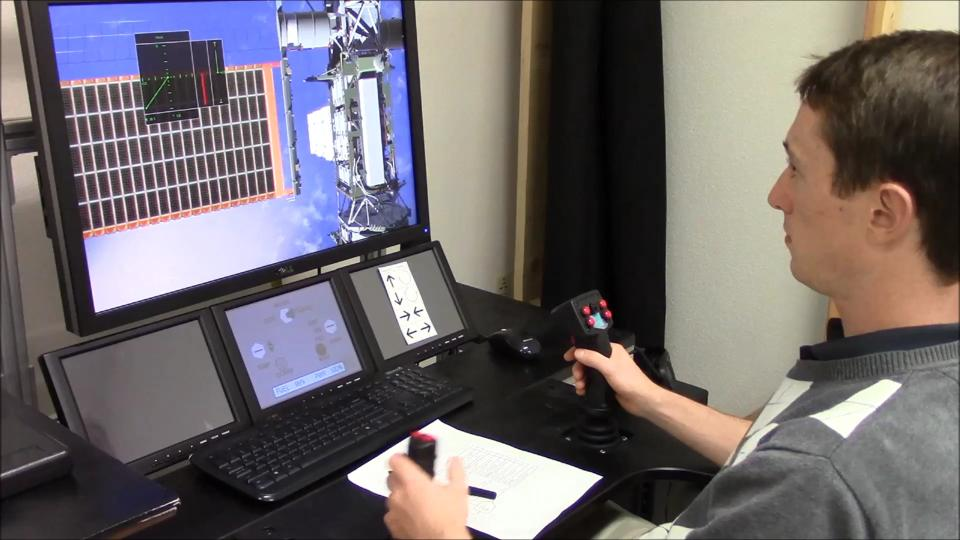
\includegraphics[width=0.8\linewidth]{figures/AR/SAFER_DangerChris.jpg}
%         \caption[Simplified Aid for EVA Rescue (SAFER) experiment subject seated in the fixed-base simulator]{A subject from the Simplified Aid for EVA Rescue (SAFER) experiment seated in the fixed-base simulator~\citep{karasinski_real-time_2016}.}
%         \label{figure:safersim}
%     \end{center}
% \end{figure}

% Our recent work includes investigations into concurrent bandwidth feedback in a four degree of freedom Simplified Aid for EVA Rescue (SAFER) task~\citep{karasinski_real-time_2016, karasinski_real-time_2017, karasinski_development_2016}.
% SAFER is a small propulsive jet pack worn during spacewalks for self-rescue~\citep{Vassigh1998}.
% Subjects were tasked with flying a SAFER simulation to perform an inspection of the International Space Station's (ISS) solar arrays.
% Subjects were initially placed 40 feet away from the solar array and were asked to close to 30 feet and hold this distance for the remainder of the task.
% They could gauge their distance from the solar array using the indicator on the guidance display and the out-the-window display.
% Subjects were then asked to inspect four waypoints on the solar array, and were given a guidance display for navigation to the waypoints.
% Two vertically arranged displays in the simulator were available to complete the task (see Figure~\ref{figure:safersim}).
% The primary display contained an out-the-window view of the solar array and, depending on which group the subject was in, one of the guidance displays.
% The secondary display located directly below the primary display portrayed information about the subject's current mode, remaining fuel, and a ``comm light.''

% \begin{figure}[tb!]
%     \begin{center}
%         \begin{subfigure}{0.49\textwidth}
%             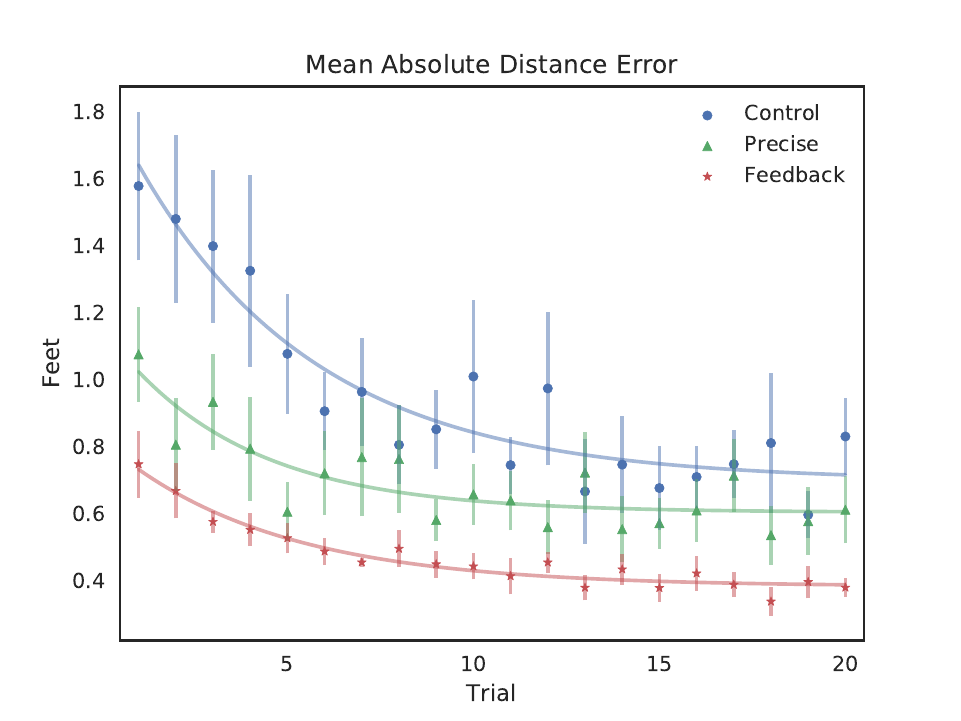
\includegraphics[width=\linewidth]{figures/AR/Group_absDistErr_clean_fit_30.png}
%             \caption[Mean absolute distance error]{Mean absolute distance error, by group.}
%             \label{figure:saferdistance}
%         \end{subfigure}\hfill
%         \begin{subfigure}{0.49\textwidth}
%             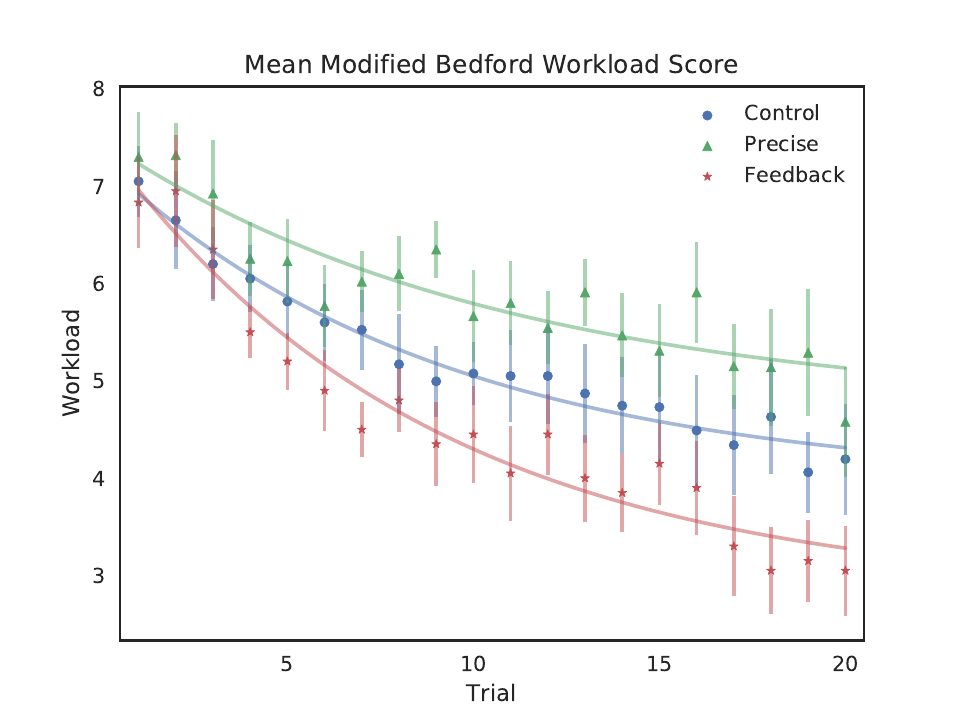
\includegraphics[width=\linewidth]{figures/AR/Group_Workload_fit_30.png}
%             \caption[Mean subjective workload rating]{Mean subjective workload rating, by group.}
%             \label{figure:saferworkload}
%         \end{subfigure}
%         \caption[Performance and workload benefits from feedback]{Subjects with concurrent bandwidth feedback (CBF) performed the best (a) and reported the lowest workload (b). Errors are the standard error of the mean~\citep{karasinski_real-time_2016}.}
%     \end{center}
% \end{figure}

% In our experiment, subjects were placed into one of three groups: a control, a high precision augmented feedback group, and a concurrent bandwidth feedback (CBF) group.
% Subjects in the high precision group were given an extra significant figure in their guidance display and an analog display which was scaled twice as large (but had half the maximum value) of their flight parameters.
% Subjects in the CBF group had two display elements which would change from a green to a red color when the subject's performance was outside a predefined range.
% Performance was measured as mean absolute distance error (MAE) and results across trials are shown in Figure~\ref{figure:saferdistance}.
% Both treatment groups performed better than the control group, with the CBF group performing the best and having the least error.
% The effects that the treatments had on workload was very different than performance, however.
% Subjects in the high precision group reported significantly more workload than the control group, while subjects in the CBF group reported significantly less workload than the control group (see Figure~\ref{figure:saferworkload}).
% The concurrent bandwidth feedback also had the added benefit of significantly reducing the amount of time required to train the subjects to their maximum skill level.
% Subjects with the CBF performed better on their first trial than subjects in the control group did on their last, which was after approximately two hours on the task.

\subsubsection{Stereoscopic Displays}
Stereoscopic displays are systems ``in which two slightly different views of a scene are provided to a viewer, one image for each eye... allow[ing] the viewer's binocular visual system to extract depth information in a scene using this disparate information''~\citep{mcintire_stereoscopic_2014}.
Without the aid of the binocular depth cue presented by stereoscopic displays, viewers are instead entirely reliant on monocular clues such relative sizing, occlusion, and motion.
One of the primary motivation for stereoscopic displays is that ``[t]he visual scene of a 3D world is a more `natural,' `ecological,' or `compatible' representation than that provided by 2D displays''~\citep{wickens_three-dimensional_1990}.
As a result of this motivation, the effects of stereoscopic displays on human performance have been extensively studied in the literature.
Several authors have attempted to classify which types of tasks may stand to benefit~\citep{mcintire_stereoscopic_2014, wickens_three-dimensional_1990, wickens_three-dimensional_1989, naikar_perspective_1998, dixon_human_2009}.
A recent review of 184 papers, for example, suggests that 60\% of studies showed some benefit of 3D stereo displays, 15\% of tasks showed unclear or mixed benefits, and 25\% of studies showed no clear benefits~\citep{mcintire_stereoscopic_2014}.
In their review, tasks involving finding/identifying/classifying objects and tasks involving real/virtual spatial manipulations of objects benefited the most, while learning/training/planning tasks were the least likely to show a benefit.

\citeauthor{kim_quantitative_1987} also performed a quantitative evaluation of perspective and stereoscopic displays in a three-axis manual tracking task.
They investigated the differences between perspective and stereoscopic displays, the elevation angle, azimuth angle, and the effects of two visual enhancements: a grid and a reference line.
They found very strong relationships between elevation and azimuth angles and tracking performance, with the best performance occurring at an elevation angle of 45 degrees and an azimuth angle of 0 degrees.
Tracking performance decreased rapidly as the azimuth angle varied, and decreased less rapidly as the elevation angle varied.
In general, they found that the stereoscopic display allowed for better tracking performance, though the inclusion of the reference line visual enhancement greatly decreased the benefit over the perspective display.
Using only two subjects, they provided some insight into intrasubject and intersubject variability.
In several instances, intrasubject variability showed 50\% changes within the same experimental condition, while intersubject variability also appeared quite large in some conditions.
\citeauthor{kim_visual_1987} repeated the evaluation of these parameters on a telerobotics pick-and-place study.
They found similar results in this second study, suggesting that their results could be generalized and that three-axis tracking performance can be correlated with pick-and-place completion time.

\citeauthor{smallman_track_2000} similarly investigated the effect of visual enhancements and 2D vs 3D displays for the development of a naval air warfare console.
Participants viewed naval and aircraft tracks in either a conventional 2D top-down display or a 3D display, and then attempted to reconstruct track positions.
They investigated the effectiveness of drop-lines and drop-shadows, and found that they significantly improved subjects ability to localize aircraft compared to when the enhancements were not present.
Furthermore, in the absence of either visual enhancement, subjects performed better with the 2D display than the 3D display.
Similar to \citeauthor{kim_quantitative_1987}, they ultimately recommended that 3D stereoscopic displays include the use of a reference or drop-line for optimal performance.

\subsubsection{Workload Measurement}
Improving performance, through some kind of feedback or other technique, often comes at the cost of increased workload, which can lead to a loss of the ability to maintain performance.
Workload was defined by \cite{hart_development_1988} as ``the perceived relationship between the amount of mental processing capability or resources and the amount required by the task.''
Having a low workload indicates that it would be easy to complete additional tasks, while having a high workload suggests that it would be difficult.

The NASA Task Load Index (NASA-TLX) is one of the most well known and commonly used subjective workload measures.
The NASA-TLX has been in use for thirty years, and has been used and validated over a large variety of tasks~\citep{hart_nasa-task_2006}.
The NASA-TLX is a multidimensional rating scale which uses the magnitude and ranking of six subscales to produce an overall estimate of subjective workload~\citep{hart_development_1988}.
The six subscales are: Mental Demand, Physical Demand, Temporal Demand, Performance, Effort, and Frustration.
Each of these scales is rated on a 0 (Very Low) to 100 (Very High) scale, with the exception of Performance, which is rated from 0 (Perfect) to 100 (Failure).
After marking a value for each of these subscales, subjects then make fifteen pairwise weightings, allowing them to rate each pair of subscales based on its perceived contribution to their overall workload.
A final, overall workload score is computed by multiplying each subscale's score by the number of times it was chosen in the pairwise weightings, adding these values, and dividing by fifteen.
As certain subscales may be more or less important than others, depending on the task being evaluated, some researchers can drop subscales or simply not compute the overall score.

In addition to subjective measures of workload, there are a variety of techniques which aim to estimate objective workload.
One of the most common objective measurement techniques is the secondary task, which requires subjects to complete the primary task, then use any spare workload to respond to an additional task~\citep{gawron_human_2008}.
Secondary tasks can provide a measure more sensitive to differences in workload and performance than a single task alone and allow for a common measure between experimental conditions~\citep{slocum1971meaningful}.
Care must be taken, however, to ensure that the secondary task does not intrude upon primary task performance~\citep{williges_behavioral_1979}.
In our previous studies, we have used a multiple choice reaction time task as an objective workload measurement.
In this secondary task, subjects are presented with several different stimuli, each of which requires a different response~\citep{lysaght_operator_1989}.
A subject's objective workload can then be inferred by either the percentage of secondary tasks which were correctly responded to within a given time, the number of secondary tasks which were correctly responded to in a trial, or both.
We have previously found this type of task to be correlated with subjective workload scales in the aforementioned SAFER task~\citep{karasinski_real-time_2017}.

\subsubsection{Summary}
Concurrent bandwidth feedback has been used in a large variety of motor control tasks, and has generally been found to improve performance.
Until recently, however, only simple tasks such as physical movements or basic pursuit tasks have been investigated.
More recent works, including the lane-keeping task by de Groot et al., and our previous work with the SAFER task, have indicated that concurrent bandwidth feedback can also be quite effective for complex tasks.
The decrease in required learning time, improved performance, and decreased workload seen in the SAFER task show that concurrent bandwidth feedback may prove to be most useful very early in training when subjects are first exposed to complex, highly dynamic tasks.
While visual concurrent bandwidth feedback has been used in a variety of tasks, no researchers have investigated its effects on a three-axis tracking task.

Despite extensive previous research, to the authors' knowledge there exists no study in the literature addressing human performance or workload changes in manual tracking tasks between traditional computer monitors and mobile, augmented reality headsets.
If operator performance while using augmented reality displays is improved--or at the very least, not degraded--then these devices could prove especially valuable in scenarios where it is impractical or otherwise difficult to provide a traditional computer interface.
There are a variety of robotics tasks, such as pick-and-place tasks, for which performance may be improved by allowing an operator the mobility to move and view the scene from whatever position is convenient at a given time.
Traditional robotics stations require the operator to remain in a single position, and typically only allow for several camera angles.
Mobile augmented reality displays allow the operator to take advantage of their ability to move through the environment, without needing to manage external cameras.

\section{Materials and Method}
\begin{figure}[b!]
    \begin{center}
        % Thanks
        % https://tex.stackexchange.com/questions/67573/tikz-shift-and-rotate-in-3d

        \newcommand{\rotateRPY}[3]% roll, pitch, yaw
        {   \pgfmathsetmacro{\rollangle}{#1}
            \pgfmathsetmacro{\pitchangle}{#2}
            \pgfmathsetmacro{\yawangle}{#3}

            % to what vector is the x unit vector transformed, and which 2D vector is this?
            \pgfmathsetmacro{\newxx}{cos(\yawangle)*cos(\pitchangle)}
            \pgfmathsetmacro{\newxy}{sin(\yawangle)*cos(\pitchangle)}
            \pgfmathsetmacro{\newxz}{-sin(\pitchangle)}
            \path (\newxx,\newxy,\newxz);
            \pgfgetlastxy{\nxx}{\nxy};

            % to what vector is the y unit vector transformed, and which 2D vector is this?
            \pgfmathsetmacro{\newyx}{cos(\yawangle)*sin(\pitchangle)*sin(\rollangle)-sin(\yawangle)*cos(\rollangle)}
            \pgfmathsetmacro{\newyy}{sin(\yawangle)*sin(\pitchangle)*sin(\rollangle)+ cos(\yawangle)*cos(\rollangle)}
            \pgfmathsetmacro{\newyz}{cos(\pitchangle)*sin(\rollangle)}
            \path (\newyx,\newyy,\newyz);
            \pgfgetlastxy{\nyx}{\nyy};

            % to what vector is the z unit vector transformed, and which 2D vector is this?
            \pgfmathsetmacro{\newzx}{cos(\yawangle)*sin(\pitchangle)*cos(\rollangle)+ sin(\yawangle)*sin(\rollangle)}
            \pgfmathsetmacro{\newzy}{sin(\yawangle)*sin(\pitchangle)*cos(\rollangle)-cos(\yawangle)*sin(\rollangle)}
            \pgfmathsetmacro{\newzz}{cos(\pitchangle)*cos(\rollangle)}
            \path (\newzx,\newzy,\newzz);
            \pgfgetlastxy{\nzx}{\nzy};
        }

        \tikzset{RPY/.style={x={(\nxx,\nxy)},y={(\nyx,\nyy)},z={(\nzx,\nzy)}}}

        \begin{tikzpicture}
            \draw[-] node at (3.5,0,0) {$x$} (-3,0,0) -- (3,0,0);
            \draw[-] node at (0,3.5/2,0) {$y$, {\color{red} $y\textprime$}} (0,-3/2,0) -- (0,3/2,0);
            \draw[-] node at (0,0,3.5) {$z$} (0,0,-3) -- (0,0,3);

            \rotateRPY{0}{-30}{0}
            \begin{scope}[draw=red, text=red,fill=red,densely dashed,RPY]
                \draw[-] node at (3.5,0,0) {$x\textprime$} (-3,0,0) -- (3,0,0);
                %\draw[-] node at (0,3.5,0) {} (0,0,0) -- (0,3,0);
                \draw[-] node at (0,0,3.5) {$z\textprime$} (0,0,-3) -- (0,0,3);
            \end{scope}
            \draw [->] (0:1.5) arc (0:-15:1.5);
            \draw[-] node at (1.7,-.2,0) {$\theta$};
        \end{tikzpicture}

        \caption[Perspective display of the coordinate frame for the tracking tasks]{Perspective display of the coordinate frame for the tracking tasks, with the $x$, $y$, and $z$ axes labeled. After rotating by $\theta$ around the y axis, the resulting reference frame of $x\textprime y\textprime z\textprime$ is also labeled.}
        \label{designdiagram}
    \end{center}
\end{figure}

In our experiment, subjects were responsible for simultaneously completing three primary tracking tasks and a two-choice secondary task.
Each axis of the tracking task was disturbed by a sum-of-sines, resulting in a random appearing signal that was difficult for the subjects to predict.
The two-choice task appeared on a screen next to the tracking task, and asked subjects to respond to either a ``LEFT'' or ``RIGHT'' command by pressing a button.
Subjects controlled the three-axes and responded to the two-choice task by using a Microsoft Xbox controller.
The subjects used the left joystick on the controller to control the $x$ and $y$ axes tracking tasks.
Subjects moved this joystick left and right to control the $x$ axis, and up and down to control the $y$ axis.
The subjects used the right joystick on the controller to control the $z$ axis.
Subjects moved this joystick up and down to control the $z$ axis.
See Figure~\ref{designdiagram} for a visualization of the coordinate frame of the primary tracking task.
Subjects used the left and right triggers on the controller to respond to the two-choice task, using the left trigger to indicate ``LEFT'' on the two-choice task, and the right trigger to indicate ``RIGHT'' on the two-choice task.

\subsection{Hypotheses}
This study assessed the influence of display type (perspective vs. stereoscopic), relative display attitude (zero degrees vs. thirty degrees), and concurrent bandwidth feedback (with vs. without) on performance and workload.
Objective performance was measured using the root-mean-square error (RMSE) of the depth ($z$) axis.
Objective workload was measured using the response time to the secondary task, and subjective workload was measured using the NASA-TLX.
It was hypothesized that:
\begin{description}[align=left]
    \item [Hypothesis 1] Concurrent bandwidth feedback will improve performance in the depth ($z$) axis for both display types, and will decrease workload.
    \item [Hypothesis 2] Stereoscopic augmented reality displays improve performance in the depth ($z$) axis, but do not affect workload.
    \item [Hypothesis 3] Rotating the display improves performance in the depth ($z$) axis for both display types, and will decrease workload.
\end{description}

\subsection{Procedure}
A total of 24 subjects (19 males, 5 females) were recruited in accordance with the University of California, Davis Internal Review Board (IRB), and subjects were not compensated.
There were 12 subjects in the 2D group, and 12 subjects in the 3D group.
Subjects were students in the University of California, Davis, College of Engineering.
All participating subjects had normal vision (no colorblindness, eyesight correctable to 20/20 vision) and full motor control of their hands.

\begin{figure}[t!]
    \begin{center}
        \begin{subfigure}{0.49\textwidth}
            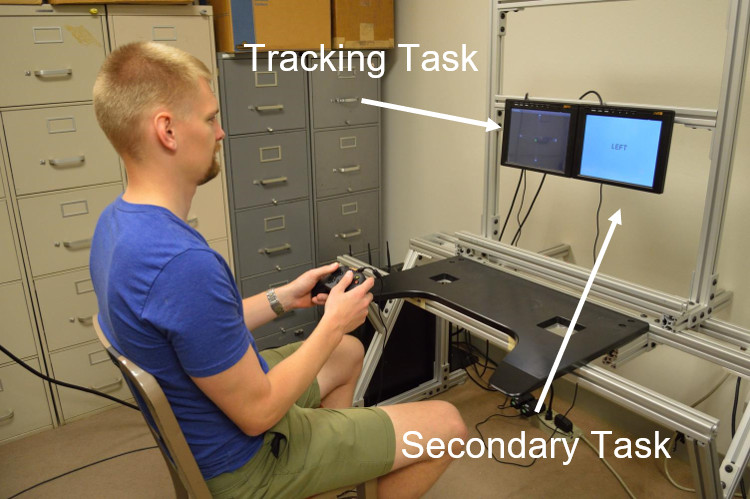
\includegraphics[width=\linewidth]{figures/AR/DSC_0801.JPG}
            \caption[2D Group]{2D Group.}
        \end{subfigure}\hfill
        \begin{subfigure}{0.49\textwidth}
            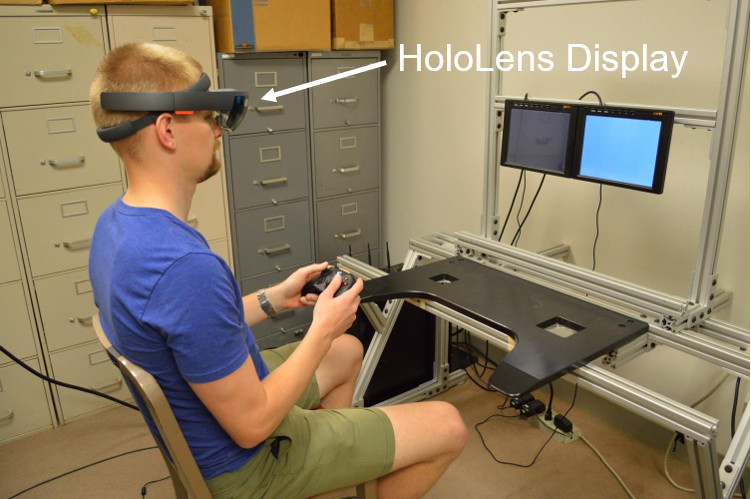
\includegraphics[width=\linewidth]{figures/AR/DSC_0803.JPG}
            \caption[3D Group]{3D Group.}
        \end{subfigure}
        \caption[The fixed-based simulator used by both groups]{The fixed-based simulator used by both groups.}%
        \label{fig:simulator}%
    \end{center}
\end{figure}

\begin{figure}[t!]
    \begin{center}
        \begin{subfigure}{0.32\textwidth}
            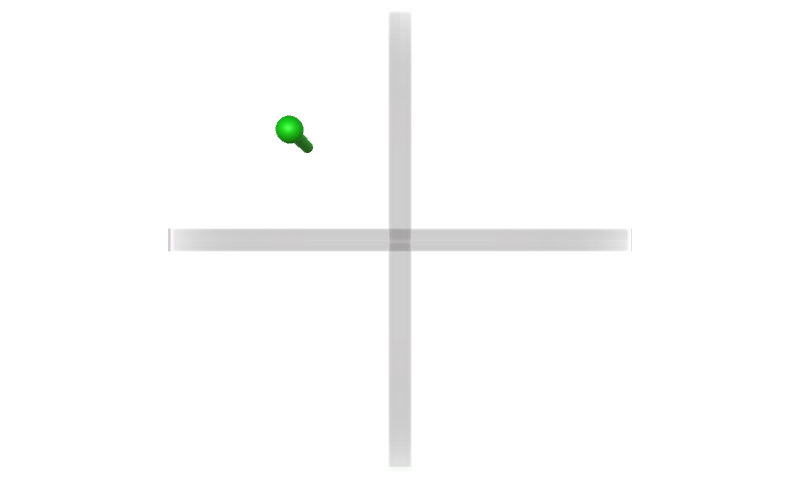
\includegraphics[trim={5cm 0 5cm 0},clip,width=\linewidth]{figures/AR/Baseline.png}
            \caption[Baseline]{Baseline.}
            \label{fig:designs_baseline}
        \end{subfigure}\hfill
        \begin{subfigure}{0.32\textwidth}
            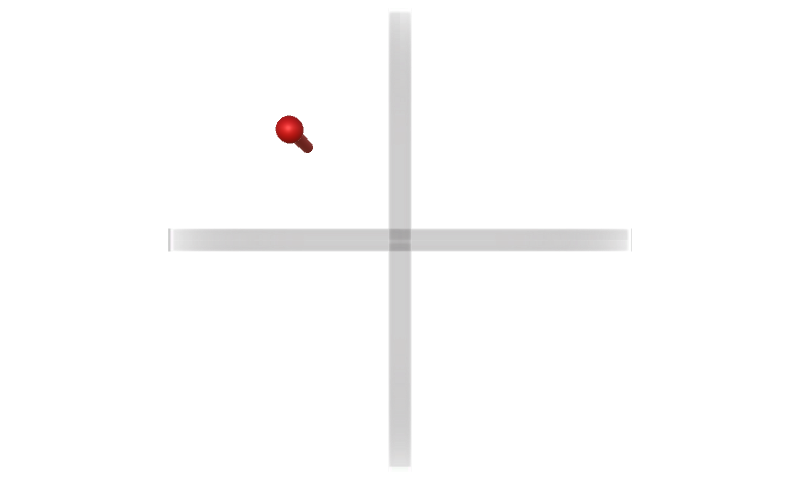
\includegraphics[trim={5cm 0 5cm 0},clip,width=\linewidth]{figures/AR/Color.png}
            \caption[Color Feedback]{Color Feedback.}
            \label{fig:designs_feedback}
        \end{subfigure}\hfill
        \begin{subfigure}{0.32\textwidth}
            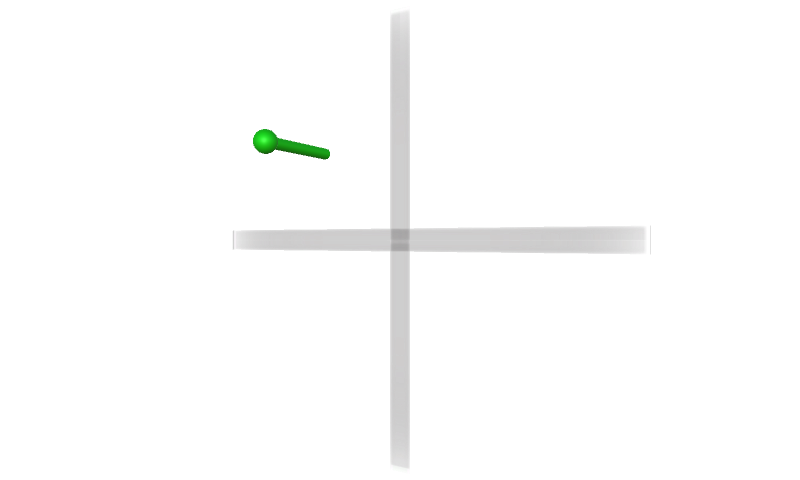
\includegraphics[trim={5cm 0 5cm 0},clip,width=\linewidth]{figures/AR/Angled.png}
            \caption[Rotated (about the $y$ axis)]{Rotated (about the $y$ axis).}
            \label{fig:designs_rotated}
        \end{subfigure}
        \caption[The three different designs in the same error state]{The three different designs in the same error state.
            (b) The color feedback has been activated here, changing the guidance target from green to red.}
        \label{fig:designs}%
    \end{center}
\end{figure}

A human-in-the-loop simulation was conducted using a fixed-base simulator (see Figure~\ref{fig:simulator}).
The simulator consisted of two 10.4 inch LCD displays.
The primary tracking task was shown on the left display, while the right display showed the two-choice secondary task.
Subjects were seated for the duration of the experiment and were placed one meter perpendicular from the center of the left display.
For subjects in the 3D group, the left LCD monitor was turned off, and the tracking task was instead displayed on the HoloLens.
For these subjects, the cross was placed at the same height as the subject's head, such that it was viewed with no relative attitude in the baseline condition (see Figure~\ref{fig:designs}).
Both groups viewed the guidance cross with a width and height of 5 inches by 5 inches.
For subjects in the HoloLen's group, the $z$ motion of the cross also could move up to 5 inches in either direction away from the center of the guidance cross.
Subjects in both groups used the same Microsoft Xbox controller and control scheme to complete the task.

The disturbance function was a sum of 13 sinusoids approximating a rectangular spectrum with a 2.0 rad/s cutoff frequency.
The disturbing force, as a function of time, $d(t)$, was
\begin{align}
    d(t) = \sum_{i=1}^{13} A_i \sin \left( w_i t + \phi_i \right)
    \label{eq:disturbance}
\end{align}
Each sine wave amplitude, frequency, and phase offset was borrowed from a similar experiment~\citep{hess_effects_1984}.
Table~\ref{sine-table} lists the sine wave amplitude, frequency, number of cycles in a 60 second run, and phase offset for each sine wave in the disturbance force.
This disturbance was the same for all subjects and trials, though the subjects were naive to this.
The $x$, $y$, and $z$ axes all experienced the same disturbance force generating function, but the $y$ axis was temporally offset by 60 seconds and the $z$ axis was offset by 120 seconds.
This allowed for a very similar generation of disturbance forces for each axis.
The RMSE of the disturbance force was normalized along each axis such that all three were the same.

\begin{table}[tb]
    \centering
    \includetable{3dar-sine-table.tex}
    \caption[Disturbance force characteristics]{The relative amplitude, frequency, number of cycles in each 60 second run, and phase offset each $i^{th}$ sine, see Equation~\ref{eq:disturbance}.}
    \label{sine-table}
\end{table}

\begin{table}[tb]
    \centering
    \includetable{3dar-designs.tex}
    \caption[The factors that were modified between the different designs]{The factors that were modified between the different designs.}
    \label{tab:designs}
\end{table}

Three designs were presented to the subjects to evaluate: a baseline design, a color-based concurrent bandwidth feedback (CBF) design, and a rotated design.
Figure~\ref{fig:designs} shows all three designs in the same error state.
The three designs were very similar, having only minor differences between each other.

The baseline design consists of a flat cross with a center target point and a green sphere error indicator.
This indicator also casts a green, variable-length rod perpendicular to the plane of the cross, which allows for a visual estimation of the error in the $z$ axis.
The $x$ axis is parallel with the horizontal cross, while the $y$ axis is parallel with the vertical cross.
The color feedback design was identical to the baseline design in every way, with the addition of visual concurrent bandwidth feedback (green or red) on the $z$ axis.
When the absolute value of the error on the $z$ axis exceeded a fixed bandwidth, the color of both the spherical indicator and the cylindrical rod changed from green to red (see Figure~\ref{fig:designs_feedback}).
When the absolute value of the error on the $z$ axis was lowered back below this fixed bandwidth, the indicator changed back to a green color (see Figure~\ref{fig:designs_baseline}).
The rotated design was identical to the baseline design, but the relative attitude of the display was rotated about the $y$ axis by 30 degrees (see Figure~\ref{designdiagram}).
This design was created to provide subjects with more visual variation in the $z$ axis, and 30 degrees was chosen after a brief pilot study.

Before entering the study, subjects were randomly placed in a display group (either the LCD monitor or HoloLens), and were then randomly placed into an order group (which consisted of Baseline-Feedback-Rotated, Feedback-Rotated-Baseline, and Rotated-Baseline-Feedback).
This order group was created to remove any order effects that might arise due to training on a given display, and follows a standard Latin squares design.
(The order of the designs was expected to be insignificant, but we will later discuss how this is not the case.)
After entering the experiment room, the subjects were familiarized with the task, three designs, NASA-TLX, and the controller through a twenty minute training session during which they were instructed to:
\begin{itemize}
    \item Minimize the displacement of their guidance target from the center
    \item Respond to the two choice task as accurately and quickly as possible
\end{itemize}

Subjects in the 3D group completed a short calibration program that adjusted the display to their interpupillary distance.
All subjects were then allowed to complete two familiarization trials, during which time they could ask questions about how the controls worked, or any other aspects of the task.
The proctor also used this time to ensure that subjects showed basic competency with the task by responding to both the tracking and two-choice tasks appropriately.
All familiarizations were done with the baseline design, regardless of which design the subjects evaluated first.

After this familiarization process, subjects completed ten trials with their first design.
After completing these trials, they answered a brief survey which asked them if the design was adequate to complete the task.
Subjects were also asked to subjectively rate their performance in a questionnaire after evaluating each design.
Subjects were asked to rate ``I found the tracking display adequate to complete the task.'' on a five point scale where 1 indicated ``Strongly Disagree'' and 5 indicated ``Strongly Agree.''
After this survey, subjects then completed a NASA-TLX workload survey.
Subjects then repeated this process with their second and third designs.
At the conclusion of the three designs, subjects were also asked to complete a preference survey which inquired into what design the subjects preferred.

\section{Results}
We conducted three-way mixed ANOVAs between display (2D or 3D), design (Baseline, Feedback, or Rotated), and starting design (Baseline, Feedback, or Rotated) with repeated measures on the design factor.
When significant effects were observed, post hoc comparisons using the Tukey Honest Significance Difference (HSD) test with a Bonferroni adjustment were completed to investigate which pairs of the factor were significant.
In order to remove learning and fatigue effects, each subject's best performing five trials in each design were averaged together to produce one average score for each subject and design.
Additionally, the first ten seconds of each sixty second trial were not included in the analysis to remove initial transient effects.

The root-mean-square error (RMSE) of the depth ($z$) axis was used to understand the differences between the three designs and the two devices.
The RMS of the disturbance signal was calculated and used to normalize the RMSE.
Under this definition, an RMSE of 1 indicates performance no better than no input, and an RMSE greater than 1 indicates quite poor performance.
It was expected that the baseline design would lead to the worst performance in the $z$ axis than the color feedback and rotated designs.
It was also expected that, due to the stereoscopic nature of the display, the HoloLens would allow for better performance than the 2D LCD monitor along $z$ axis.

\begin{figure}[tb!]
    \begin{center}
        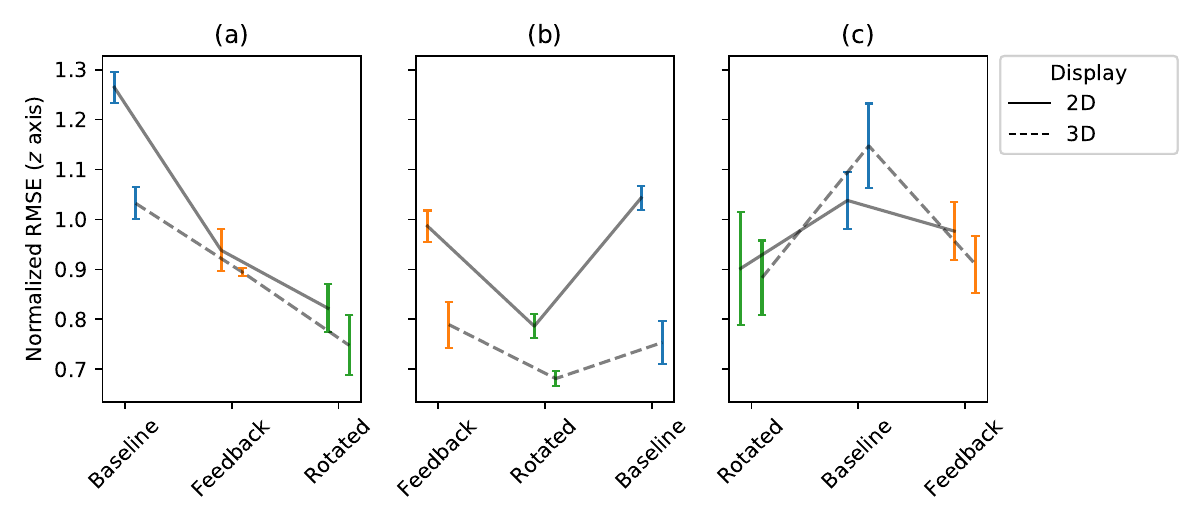
\includegraphics[height=7cm]{figures/AR/x_design_y_zrmse_col_startdesign_hue_device.png}
        \caption[The resulting normalized RMSE along the $z$ axis]{The resulting normalized RMSE along the $z$ axis. Subjects started in either the (a) Baseline, (b) Feedback, or (c) Rotated design.}
        \label{fig:zrmseanovas}
    \end{center}
\end{figure}

Results of the ANOVA on the $z$ axis RMSE showed significant effects for design ($F(2, 36)=84.92, p<.001$), device ($F(1, 18)=7.22, p<0.015$), and start design ($F(2, 18)=4.81, p<0.021$).
The ANOVA also showed a significant interaction effect between design and starting design ($F(4, 36)=8.55, p<0.0001$), and a three way interaction between design, device, and starting design ($F(4, 36)=5.57, p<0.002$).
Further investigation into the effect of starting design using pairwise comparisons showed significance differences between subjects that started in the concurrent bandwidth feedback group and those in the baseline ($p<0.001$) or rotated ($p<0.001$) designs, but no difference between subjects that started in the baseline and rotated designs ($p>.38$).
The difference in performance between design, device, and starting design can be seen in Figure~\ref{fig:zrmseanovas}.

Due to the unanticipated but significant interaction effects in the starting design factor, the remainder of the analysis is split between subjects who started with the concurrent bandwidth feedback design and those that did not (e.g., those that started in the baseline or rotated design).
For subjects that started in the CBF design, there was a significant effect of design ($F(2, 12)=21.65, p<.0001$), a significant effect of display ($F(1, 6)=36.73, p<0.001$), and a significant interaction effect between design and device ($F(2, 12)=5.42, p<0.021$).
For subjects that did not start in the CBF design, there was a significant effect of design ($F(2, 28)=38.70, p<.0001$), but no significant effect or display ($F(1, 14)=1.03, p>0.32$), and no interaction effect ($F(2, 12)=0.03, p>0.97$).
The resulting difference between subjects who started in the CBF design and those who did not is presented in Figure~\ref{fig:zrmseanovas2}.
For subjects who did not start in the CBF design, display had no significant effect, and subjects performed best in the rotated design, followed by the feedback design and finally the baseline design.
Subjects who started in the CBF design performed significantly better in the 3D display than the 2D displays, and performed best in the rotated design, but comparably between the feedback and baseline designs.

\begin{figure}[tb!]
    \begin{center}
        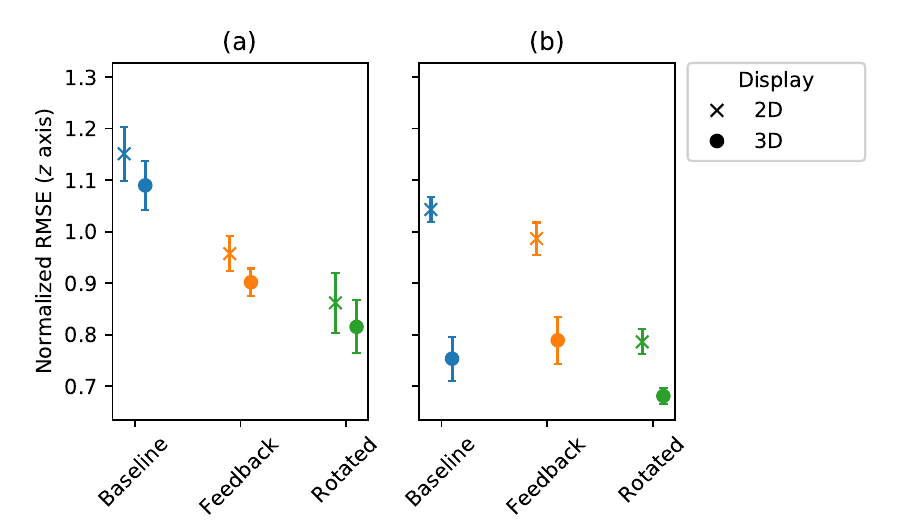
\includegraphics[height=7cm]{figures/AR/x_design_y_zrmse_hue_device_col_cbf_first.png}
        \caption[The resulting normalized RMSE along the $z$ axis]{The resulting normalized RMSE along the $z$ axis, grouping by subjects that started (a) without or (b) with feedback.}
        \label{fig:zrmseanovas2}
    \end{center}
\end{figure}

The NASA-TLX was used to measure differences in subjective workload, and the reaction time to the secondary task was used to measure differences in objective workload between design, device, and starting design.
There were no significant effects, nor interaction effects, found in the ANOVA for design, device, or starting design for the NASA-TLX measurements.
There was a significant effect of design ($F(2, 36)=7.93, p<0.0014$) for the reaction time to the secondary task, though the magnitude of this effect was very small between designs (less than 100 ms difference) and was not significant during Tukey HSD tests.
In general, there were no significant effects found for workload measurements.

\section{Discussions and Conclusion}
To summarize these results, there were significant effects found in the $z$ axis RMSE for design, with subjects generally performing the best using the rotated design, followed by the CBF design, and performing worst with the baseline design.
There were significant effects found for the factors of device and starting design, though these must be interpreted carefully.
Subjects who started with concurrent bandwidth feedback performed better than subjects who did not.
We believe that this result reinforces that found in our prior SAFER experiment, where subjects who were exposed to the CBF early on learned the task better than those who were not exposed~\citep{karasinski_real-time_2016,karasinski_development_2016,karasinski_real-time_2017}.
An interesting effect of this exposure is that, after learning the task with CBF, subjects continued on to perform significantly better in the baseline condition than those subjects that did not start in the CBF design.

Subjects who started in the CBF design and who were wearing the HoloLens appear to have used the CBF to better learn the depth cue presented in the stereoscopic display.
These subjects continued to perform significantly better than subjects who started with the CBF design but without the stereoscopic display when they continued to the baseline design.
This indicates that even a brief exposure to the concurrent bandwidth feedback was sufficient to induce improved performance in the baseline design.
Additionally, this also suggests that well trained subjects could perform better using the stereoscopic display compared with the traditional display, but that subjects who were still learning the task could not take advantage of the additional depth cues provided by the display.
Finally, there were no significant effects found for the NASA-TLX measurements, and there were significant but small effects found between the designs for reaction time.

In summary, we find partial agreement with all of our hypotheses in respect to the performance aspects of our experiment, while the workload was essentially unaffected by all of our experimental factors.
For Hypothesis 1, subjects who completed the baseline design before the CBF design performed better in the CBF design, while subjects who completed the CBF design before the baseline performed approximately the same in both designs.
This indicates that CBF can both improve performance compared to a baseline design, and better train subjects such that, even after brief exposure, the feedback is no longer required.
Workload was unaffected by the CBF.
For Hypothesis 2, subjects who started in the CBF design appear to have better learned the task and used the CBF to learn to interpret the depth cue provided by the stereoscopic display.
Subjects who were not initially exposed to this feedback were unable to exploit the display, and did not perform significantly better than subjects without the display.
For Hypothesis 3, subjects in the rotated design did perform better than those in the baseline design and appeared to be able to use this view to better interpret the depth of the target.

These results suggest that 3D displays such as the HoloLens have the potential to improve performance, but that simply donning a 3D display is not in itself wholly sufficient for improvement.
Subjects performed the tracking task better when we exposed them to CBF early in the experiment, and were able to use the depth cues provided by the 3D display to sustain this improvement when the feedback was removed.
These subjects achieved the best performance that we observed in this experiment, suggesting that the combination of CBF and 3D displays is an effective training technique for optimal performance.
The rotated design generally resulted in excellent performance by all subjects, which suggests that a direct ($\theta=0$) view should be avoided for three-axis tracking tasks.
Care must be taken to provide subjects with the feedback required to adequately complete the task, and subjects should not expect to perform better simply because they have 3D displays.

% \section*{Acknowledgments}
% The authors would like to thank all the subjects for volunteering to take part in the study.
% This work was supported by the Link Foundation's Modeling, Simulation, and Training Fellowship.
